\section{Extended version}
\label{specification-extended}

Section \ref{specification-original} describes a benchmark that can be used to compare performance of different tools. This Sections extends this benchmarking conecpt by characterizing instance models and queries by metrics, and evaluate which tools are the most sensitive to which metrics. 

\subsection{Overview}
\label{sec:benchmark_overview}
The aim of our metrics and benchmarking scenarios is to give a precise mechanism for identifying key factors in selecting between different query evaluation technologies.

The presented metrics for our evaluation (see in~\autoref{sec:benchmark-metrics}) were constructed based on a set of already and widely used metrics, extended with two more specific ones that aims to give a gross upper bound on the cost of query evaluation.

For the benchmark scenario we opted for a simple execution schema that represents a batch validation scenario. This is the same as the first two phase of the original benchmark. See \figref{fig:phases} and \autoref{sec:phases} for a description of the \emph{read} and \emph{check} phases. 


\subsection{Metrics}
\label{sec:benchmark-metrics}

Our investigation relies on a selection of metrics that quantitatively describe
the task of a certain query, independently of the actual strategy or technological solution
that provides the query results. Broadly speaking, such a querying task consist
of (a) an instance model, (b) a query specification that defines what results
should be yielded, (c) a runtime context in which the queries are evaluated,
such as the frequency of individual query evaluations and model manipulation
inbetween.

The metrics discussed in the following, characterize instance models, queries or their combination, without characterizing a unique property of a specific graph/query description language or environment. Most of these metrics have previously been defined by other sources, while others are newly proposed in this paper.

\subsubsection{Metrics for Instance Model Only}
Clearly, properties of the instance model may have a direct effect on query
performance, e.g.\ querying larger models may consume  more resources.

% do NOT press Esc+Q !!! (or re-wrap comment!)
A first model metric is model size, which can be defined either as the
number of objects (metric \code{countNodes}), the number of references (edges)
between objects (\code{countEdges}), the number of attribute value assignments
(not used in the paper);
%\code{countValueAssignments} 
or some combination of
these three, such as their sum (\code{countTriples}), which is basically the
total number of model elements / RDF triples. This is complemented by the number
of different classes the objects in the model belong to (\code{countTypes}), and
the instance count distribution of the classes. %( TODO todo \todo{todo}).
Additional important model metrics characterize the distribution of the
out-degrees and in-degrees (the number of edges incident on an object),
particularly the maximum and average degrees (\code{maxInDegree},
\code{maxOutDegree}, \code{avgInDegree} and \code{avgOutDegree}).
 
The metrics discussed above have been defined e.g.\ in~\cite{COLD2012-analysis-DBLP:conf/semweb/StarkaSM12}, along with other
metrics such as the relative frequencies of the edge label sequences of directed
paths of length 2 or 3.
 
\subsubsection{Metrics for Query Specification Only}
The query specification is a decisive factor of performance as well, as complex
queries may be costly to evaluate. Such query metrics can be defined separately,
in several query formalisms. Due to the
close analogies between graph patterns and SPARQL queries, we can consider these
metrics applying to graph pattern-like queries in general. This allows us to
formulate and calculate metrics expressed on the graph patterns interpreted by
\eiq{}, and characterize the complexity of the equivalent SPARQL query with
the same metric value.

As superficial metrics for graph pattern complexity, we propose the number of
variables (\code{numVariables}) and the number of parameter variables
(\code{numParameters}); the number of pattern edge constraints
(\code{numEdgeConstraints}) and the number of attribute check constraints
(\code{numAttrChecks}); finally the maximum depth of nesting NACs
(\code{nestedNacDepth}). Some of these are similar/equivalent to 
SPARQL query metrics defined in~\cite{SPLODGE}. Other metrics proposed
by~\cite{SPLODGE} are mostly aimed at measuring special properties relevant to
certain implementation strategies.

\subsubsection{Metrics for Combination of Query and Instance Model}
The following two metrics (defined previously in literature) characterize the
query and the instance model together.

The most trivial such metric is the cardinality of the query results (metric
\code{countMatches}); intuitively, a query with a larger result set typically
takes longer to evaluate on the same model, while a single query is typically
more expensive to evaluate on models where it has more matches. The metric
\code{selectivity} is proposed by~\cite{SPLODGE}, is the ratio of the
number of results to the number of model elements (i.e.\ 
$countMatches/countTriples$).


\subsubsection{New Metrics for Assessing Query Evaluation Difficulty}
We propose two more metrics that take query and instance model characteristics into account. 
Our aim is to provide a gross upper bound on
the cost of query evaluation. We consider all \emph{enumerable} constraints in
the query, for which it is possible to enumerate all tuples of variables
satisfying it; thus edge constraints and pattern composition are enumerable,
while NACs and attribute checks in general are not. At any given state of
evaluation, a hypothetical search-based query engine has either already
identified a single occurrence of an enumerable constraint $c$ (e.g.\ a single
instance of an edge type for the corresponding edge constraint), or not; there
are therefore $\abs{c}+1$ possible cases for $c$, where $\abs{c}$ is the number
of different ways that $c$ can be satisfied in the model. This gives
$\prod_{c}{1+\abs{c}}$ as the overestimate of the search space of the query
evaluator. To make this astronomical figure manageable, we propose the absolute
difficulty metric (\code{absDifficulty}) as the logarithm of the search space
size, i.e.\ $ln\prod_{c}{(1+\abs{c})} = \sum_{c}{ln(1+\abs{c})}$.
 
The result size is a lower bound of query evaluation cost, since query
evaluation takes at least as much time or memory as the number of results. It is
therefore expected that queries with a high number of matches also score high on
the absolute difficulty metric. To compensate for this, the relative difficulty
metric (\code{relDifficulty}) is defined as
$ln\frac{\prod_{c}{(1+\abs{c})}}{1+countMatches} = \sum_{c}{ln(1+\abs{c})} -
ln(1+countMatches)$, expressing the logarithm of the ``challenge'' the query
poses -- this is how much worse a query engine can do than the lower bound. 
If the relative metric is a low figure, than the cost of query evaluation will not
be much worse than the optimum, regardless of the query evaluation strategy. It
can be easily shown that if a part of a graph pattern is extracted as a helper
pattern that is used via pattern composition, then the sum of the relative
difficulties of the two resulting patterns will be the same as the relative
difficulty of the original pattern. This suggests that this metric should be
treated as additive over dependent queries, and also that it is worth extracting
common parts of multiple patterns into reusable helper patterns.

\subsection{Modified Metamodel}

\begin{figure}[htb]
\begin{center}
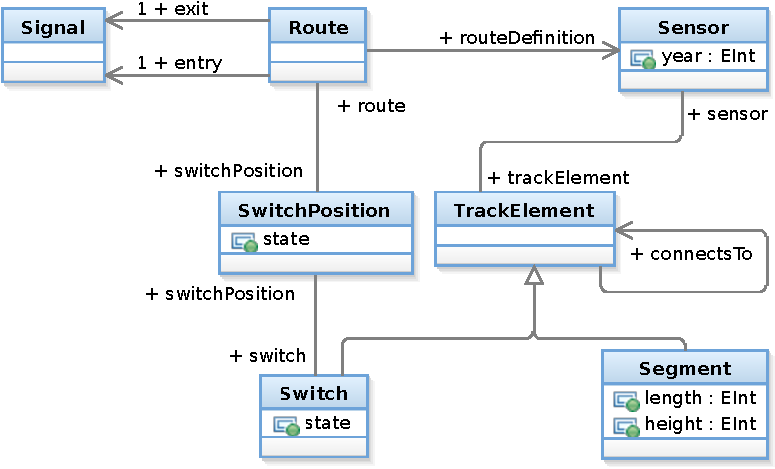
\includegraphics[width=12cm]{figures/TrainMMMet.pdf}
\caption{The railway metamodel (metrics version).}
\label{fig:metamodel-met}
\end{center}
\end{figure}

The metamodel used for merics evaluation is depicted in \figref{fig:metamodel-met}. This is similar to the one presented in \autoref{sec:domain}, but cardinality constraints are mostly omitted, and \emph{height} and \emph{year} integer attributes are introduced for classes Segment and Sensor respectively. This gives higher freedom for the instance model generator, and more queries can be defined for attribute checks.

\subsection{Instance Models for the Modified Metamodel}
\label{sec:benchmark-models}

Models are characterized by their size and structure. Here size refers to the cardinalities of node and edge types. The fact that increasing model size tends to increase the cost of queries is intuitively self evident (and also empirically confirmed e.g.\ by our previous experiments~\cite{icgt08-bhrv,models10}). Handling large models in real life is a great chellenge, but model structure (that determines which nodes are connected to each other by which edges) must also be taken into account, which here means edge distribution of nodes. Different edge distributions also present in real-world networks: the internet or protein-protein interaction networks show \emph{scale-free} characteristics~\cite{barabasi_network_2004}, while in other areas self-healing algorithms for \emph{binomial computer networks} are studied~\cite{binomial-self-healing}. Average degree can impact performance greatly, which is a typical property of different model kinds. For example, software models have usually nodes with \emph{low degree}, while social models are usually \emph{dense graphs}. 

We have conducted the experiments on synthetic models, generated automatically
with our model builder, belonging to three \concept{model families}  (without
comparing them directly to real world ones, leaving it as a future work). All
generated models within a family have the same approximate size; though there is
some random variation due to the generation process (see later), with low
standard deviation (e.g.\ measured as 0.3\% in family $A$).  Family $A$ models are relatively dense graphs
(\texttildelow 26 edges/nodes, i.e.\ metric \code{avgOutDegree}) with 1.8 million
total model elements (metric \code{numTriples}); family $B$ models are equally
dense, but are scaled back to only 113 thousand elements; finally family $C$
models have almost 1.3 million model elements that form a relatively sparse
graph ($8.4-8.7$ edges/nodes).

Each model of a family has the same (expected) number of instances for any given
type. However, these models of the same size still differ in their internal
\concept{structure}. Given the cardinalities of each type, our generator first
created the instance sets of node types, along with generating attribute values
according to an associated distribution. Then for each edge type, the generator
created edge instances (with the given expected cardinality) between instances
of the source type and instances of the target type. The structure of the graph
is induced by the method of choosing which source node and which target node to
connect. We have applied the following four methods, each taking as input the
set $S$ of source node candidates, the set $T$ of target node candidates, and
the expected cardinality $e$ of the edge type. %\begin{description}

  \emph{Binomial case.} Inspired by the well-known Erdős-Rényi model of random
  graphs~\cite{erdos1960erg}, the first approach is to take each pair of source and
  target nodes, and draw an edge between them with a given probability $p$. This makes the
  expected cardinality of edges $e = p \times \abs{S} \times \abs{T}$, thus $p$
  is chosen as $\frac{e}{\abs{S} \times \abs{T}}$. The degrees of nodes will be
  binomially distributed, e.g.\ out-degrees with parameters $\abs{T}$ and $p$.
  
  \emph{Hypergeometric case.} While the previous solution ended up with a
  random number of edges (with expected value $e$), this slightly different
  approach will generate exactly $e$ edges, by taking each pair of source and
  target nodes, and randomly selecting $e$ from them into the graph. The degrees
  will be hypergeometrically distributed, e.g.\ out-degrees with parameters
  $\abs{S} \times \abs{T}$, $\abs{T}$ and $e$.
    
  \emph{Regular case.} In software engineering models, one often finds for a
  given edge type that out-degrees of all nodes of the source type are roughly
  equal, and the same is true for in-degrees. This motivated a method that tries
  to uniformly (but randomly) divide $e$ edges between the source nodes, so that
  the difference between any two out-degrees is at most 1; while also dividing
  the same edges between the target nodes, with a similar restriction on
  in-degrees.
  
  \emph{Scale-free case.} It has been observed in many different disciplines
  that degree distributions of certain large graphs follow a power law,
  especially growing / evolving graphs with the \emph{preferential attachment}
  property (a new edge is more likely to connect to a node which already has a
  higher degree). We have used a variant of the preferential attachment
  bipartite graph generator algorithm of~\cite{RandomNetworkGeneration2005} to
  generate the connections from source nodes to target nodes.
 
The four generation methods induced significantly different degree
distributions. 
This and other differences are shown in \autoref{tbl:instance_metric_values}.
 
One-to-many relationships were treated in a special way to meet the multiplicity
restriction. In particular, a single top-level container element (not depicted
in the metamodel figure, neither involved in any queries) was used to contain
all elements; it therefore has an outgoing containment edge for every other
object, thereby ``polluting'' the \code{maxOutDegree} metric.

\begin{table*}[tp]
	\centering
	\resizebox{\textwidth}{!}{
	\begin{tabular}{|c|l|r|r|r|r|r|r|r|r|}%{|l|c|c|c|c|c|c|c|c|c|c|}
	\hline 
	\textbf{Model Family} & \textbf{Model structure} & \textbf{countNodes} & \textbf{countEdges} & \textbf{countTriples} & \textbf{countTypes} & \textbf{avgOutDegree} & \textbf{avgInDegree} & \textbf{maxOutDegree} & \textbf{maxInDegree}\\ \hline
	A & Regular & 63289 & 1646386 & 1811752 & 7 & 26.01 & 26.01 & 63288 & 44\\ \hline
	A & Binomial & 63289 & 1649179 & 1814545 & 7 & 26.06 & 26.06 & 63288 & 69\\ \hline
	A & HyperGeo & 63289 & 1646386 & 1811752 & 7 & 26.01 & 26.01 & 63288 & 74\\ \hline
	A & Scalefree & 63289 & 1660033 & 1825399 & 7 & 26.23 & 26.23 & 63288 & 10390\\ \hline
	
	B & Regular & 3954 & 102839 & 113170 & 7 & 26.01 & 26.01 & 3953 & 44\\ \hline
	B & Binomial & 3954 & 102984 & 113315 & 7 & 26.05 & 26.05 & 3953 & 64\\ \hline
	B & HyperGeo & 3954 & 102839 & 113170 & 7 & 26.01 & 26.01 & 3953 & 69\\ \hline
	B & Scalefree & 3954 & 96029 & 106360 & 7 & 24.29 & 24.29 & 3953 & 918\\ \hline
	
	C & Regular & 120001 & 1040000 & 1280001 & 7 & 8.67 & 8.67 & 120000 & 13\\ \hline
	C & Binomial & 120001 & 1041323 & 1281324 & 7 & 8.68 & 8.68 & 120000 & 30\\ \hline
	C & HyperGeo & 120001 & 1040000 & 1280001 & 7 & 8.67 & 8.67 & 120000 & 29\\ \hline
	C & Scalefree & 120001 & 1012858 & 1252859 & 7 & 8.44 & 8.44 & 120000 & 8929\\ \hline
	
	\end{tabular} 
	}
	\caption{Values of model metrics on the generated instance models.}
	\label{tbl:instance_metric_values}
	\end{table*}


\subsection{Benchmark Queries}
\label{sec:benchmark-queries}

Based on the previously defined metrics for query specification and based on the
metamodel, six series of model query specifications were systematically
constructed. Each query series includes four to seven model queries that aim to
be different in only one of the defined model query metrics. Executing a query
series on the same model and tool results in a data series that shows how the
tool is scalable according to the represented model metric.

\subsubsection{\code{Locals} Query Series for the \code{numVariables} Metric}
Five queries were defined, where each one includes the same number of edge
constraints, but the number of local variables increases. 

It can be realized using the \code{Segment} type and \code{connectsTo}
reference, so it means that only one node type and reference type is used in
these patterns and the focus is on the structure of the patterns. The simple
graph based visualisation of these pattern structures is shown in \figref{fig:aselocals},
where the node drawn with empty circle represents the
single pattern parameter.

\tikzstyle{every node}=[circle, draw, fill=black, inner sep=0pt, minimum
							width=4pt, scale=0.5, node distance=2cm]
\begin{figure}[ht]
	\centering
	\begin{tikzpicture}[->,>=stealth',shorten >=1pt,auto, thick,main
	  node/.style={circle,fill=black,draw,font=\sffamily\Large\bfseries,inner
	  sep=0pt, minimum width=4pt}]
	
	  \node[main node] (3) [] {3};
	  \node[main node, fill=white, minimum width=12pt] (1) [above left of=3]{};
	  \node[main node] (2) [above right of=3] {2};
	
	  \path[every node/.style={font=\sffamily\small}]
	    (1) edge node {} (2)
	        edge [bend right] node {} (3)
	    (2) edge [bend right] node [right] {} (1)
	        edge node {} (3)
	    (3) edge node [right] {} (1)
	        edge [bend right] node {} (2);
	\end{tikzpicture}
	\hspace{3mm}
	\begin{tikzpicture}[->,>=stealth',shorten >=1pt,auto,thick,main
	  node/.style={circle,fill=black,draw,font=\sffamily\Large\bfseries,inner
	  sep=0pt, minimum width=4pt}]
	
	  \node[main node, fill=white, minimum width=12pt] (1) []{};
	  \node[main node] (2) [right of=1] {2};
	  \node[main node] (3) [below of=1] {3};
	  \node[main node] (4) [right of=3] {4};
	
	  \path[every node/.style={font=\sffamily\small}]
	    (1) edge node {} (2)
	        edge node {} (4)
	    (2) edge node {} (4)
	    (3) edge node {} (1)
	        edge node {} (2)
	    (4) edge node {} (3)
	        ;
	\end{tikzpicture}
	\hspace{3mm}
	\begin{tikzpicture}[->,>=stealth',shorten >=1pt,auto,node distance=3cm,
	  thick,main
	  node/.style={circle,fill=black,draw,font=\sffamily\Large\bfseries,inner
	  sep=0pt, minimum width=4pt}]
	
	  \node[main node, fill=white, minimum width=12pt] (1) []{};
	  \node[main node] (2) [right of=1] {2};
	  \node[main node] (3) [right of=2] {3};
	  \node[main node] (4) [below of=1] {4};
	  \node[main node] (5) [right of=4] {5};
	
	  \path[every node/.style={font=\sffamily\small}]
	    (1) edge node {} (2)
	    (2) edge node {} (3)
	        edge node {} (4)
	    (3) edge node {} (5)
	    (4) edge node {} (1)
	    (5) edge node {} (4)
	        ;
	\end{tikzpicture}
	\hspace{3mm}
	\begin{tikzpicture}[->,>=stealth',shorten >=1pt,auto,node distance=3cm,
	  thick,main
	  node/.style={circle,fill=black,draw,font=\sffamily\Large\bfseries,inner
	  sep=0pt, minimum width=4pt}]
	
	  \node[main node, fill=white, minimum width=12pt] (1) []{};
	  \node[main node] (2) [right of=1] {2};
	  \node[main node] (3) [below right of=2] {3};
	  \node[main node] (4) [below left of=3] {4};
	  \node[main node] (5) [left of=4] {5};
	  \node[main node] (6) [below left of=1] {6};
	
	  \path[every node/.style={font=\sffamily\small}]
	    (1) edge node {} (2)
	    (2) edge node {} (3)
	    (3) edge node {} (4)
	    (4) edge node {} (5)
	    (5) edge node {} (6)
	    (6) edge node {} (1)
	        ;
	\end{tikzpicture}
	\hspace{3mm}
	\begin{tikzpicture}[->,>=stealth',shorten >=1pt,auto,node distance=3cm,
	  thick,main
	  node/.style={circle,fill=black,draw,font=\sffamily\Large\bfseries,inner
	  sep=0pt, minimum width=4pt}]
	
	  \node[main node, fill=white, minimum width=12pt] (1) []{};
	  \node[main node] (2) [right of=1] {2};
	  \node[main node] (3) [right of=2] {3};
	  \node[main node] (4) [below right of=3] {4};
	  \node[main node] (5) [below left of=4] {5};
	  \node[main node] (7) [below left of=1] {7};
	  \node[main node] (6) [below right of=7] {6};
	
	  \path[every node/.style={font=\sffamily\small}]
	    (1) edge node {} (2)
	    (2) edge node {} (3)
	    (3) edge node {} (4)
	    (4) edge node {} (5)
	    (5) edge node {} (6)
	    (6) edge node {} (7)
	        ; 
	\end{tikzpicture}
	\caption{The \codeCap{Locals} patterns.}
	\label{fig:aselocals}
\end{figure}	

\subsubsection{\code{Refs} Query Series for the \code{numEdgeConstraints}
Metric}
%Like the query series for metric \code{numVariables}, 
The \code{Refs} query series is
also constructed based on the \code{Segment} type and \code{connectsTo}
reference. 

Here, the number of edge constraints increases along the series, but
the number of local variables is constant in all of the generated four queries.
The visualisation of these pattern structures is shown in \figref{fig:aserefs}. 

\begin{figure}[ht]
	\centering
	\begin{tikzpicture}[->,>=stealth',shorten >=1pt,auto, thick,main
	  node/.style={circle,fill=black,draw,font=\sffamily\Large\bfseries,inner
	  sep=0pt, minimum width=4pt}]
	
	  \node[regular polygon, regular polygon sides=5, minimum
	  size=3cm,name=x,fill=white, draw=none] at (0,0) {}; 
	  \foreach \corner in {1,2,...,5}
	  	  \ifthenelse{\equal{\corner}{1}}{
			\node[fill=white,circle,minimum width=12pt] (\corner) at (x.corner \corner){}
	  	  	}{
			\node[circle,minimum width=12pt] (\corner) at (x.corner \corner){}
	  	  	};
	
	  \path[every node/.style={font=\sffamily\small}]
	    (1) edge node {} (2)
	    (2) edge node {} (3)
	    (3) edge node {} (4)
	    (4) edge node {} (5)
	  ;
	\end{tikzpicture}
	\hspace{3mm}
	\begin{tikzpicture}[->,>=stealth',shorten >=1pt,auto,thick,main
	  node/.style={circle,fill=black,draw,font=\sffamily\Large\bfseries,inner
	  sep=0pt, minimum width=4pt}]
	
	  \node[regular polygon, regular polygon sides=5, minimum
	  size=3cm,name=x,fill=white, draw=none] at (0,0) {}; 
	  \foreach \corner in {1,2,...,5}
	  	  \ifthenelse{\equal{\corner}{1}}{
			\node[fill=white,circle,minimum width=12pt] (\corner) at (x.corner \corner){}
	  	  	}{
			\node[circle,minimum width=12pt] (\corner) at (x.corner \corner){}
	  	  	};
	
	  \path[every node/.style={font=\sffamily\small}]
	    (1) edge node {} (2)
	    (2) edge node {} (3)
	    (3) edge node {} (4)
	    (4) edge node {} (5)
	
	    (1) edge node {} (3)
	  ;
	\end{tikzpicture}
	\hspace{3mm}
	\begin{tikzpicture}[->,>=stealth',shorten >=1pt,auto,node distance=3cm,
	  thick,main
	  node/.style={circle,fill=white,draw,font=\sffamily\Large\bfseries,inner
	  sep=0pt, minimum width=4pt}]
	
	  \node[regular polygon, regular polygon sides=5, minimum
	  size=3cm,name=x,fill=white, draw=none] at (0,0) {}; 
	  \foreach \corner in {1,2,...,5}
	  	  \ifthenelse{\equal{\corner}{1}}{
			\node[fill=white,circle,minimum width=12pt] (\corner) at (x.corner \corner){}
	  	  	}{
			\node[circle,minimum width=12pt] (\corner) at (x.corner \corner){}
	  	  	};
	
	  \path[every node/.style={font=\sffamily\small}]
	    (1) edge node {} (2)
	    (2) edge node {} (3)
	    (3) edge node {} (4)
	    (4) edge node {} (5)
	
	    (1) edge node {} (3)
	    (2) edge node {} (4)
	  ;
	        
	\end{tikzpicture}
	\hspace{3mm}
	\begin{tikzpicture}[->,>=stealth',shorten >=1pt,auto,node distance=3cm,
	  thick,main
	  node/.style={circle,fill=black,draw,font=\sffamily\Large\bfseries,inner
	  sep=0pt, minimum width=4pt}]
	
	  \node[regular polygon, regular polygon sides=5, minimum
	  size=3cm,name=x,fill=white, draw=none] at (0,0) {}; 
	  \foreach \corner in {1,2,...,5}
	  	  \ifthenelse{\equal{\corner}{1}}{
			\node[fill=white,circle,minimum width=12pt] (\corner) at (x.corner \corner){}
	  	  	}{
			\node[circle,minimum width=12pt] (\corner) at (x.corner \corner){}
	  	  	};
	
	  \path[every node/.style={font=\sffamily\small}]
	    (1) edge node {} (2)
	    (2) edge node {} (3)
	    (3) edge node {} (4)
	    (4) edge node {} (5)
	    (1) edge node {} (3)
	    (2) edge node {} (4)
	    (3) edge node {} (5)
	  ;
	  
	  
	\end{tikzpicture}
	\caption{The \codeCap{Refs} patterns.}
	\label{fig:aserefs}
\end{figure}



\subsubsection{\code{Params} and \code{ParamCircle} Query Series for the
\code{numParameters} Metric} Two series of queries were constructed for this
metric, because of performance reasons. The \code{Params} query series is the more
complex and some tools exceed the time limit in the benchmark. The
\code{ParamsCircle} query series is a simplification of the \code{Params}
series.

The goal of this constructed query series is to create patterns with the same
body, but with an increasing number of parameters. The first of these queries
(returning one parameter) is shown in \figref{fig:aseparams}, where the
parameter is the blue object. Other queries use the same body, but add sen1,
then sen2, then other variables to the parameter list.

\begin{figure}[htb]
\begin{center}
    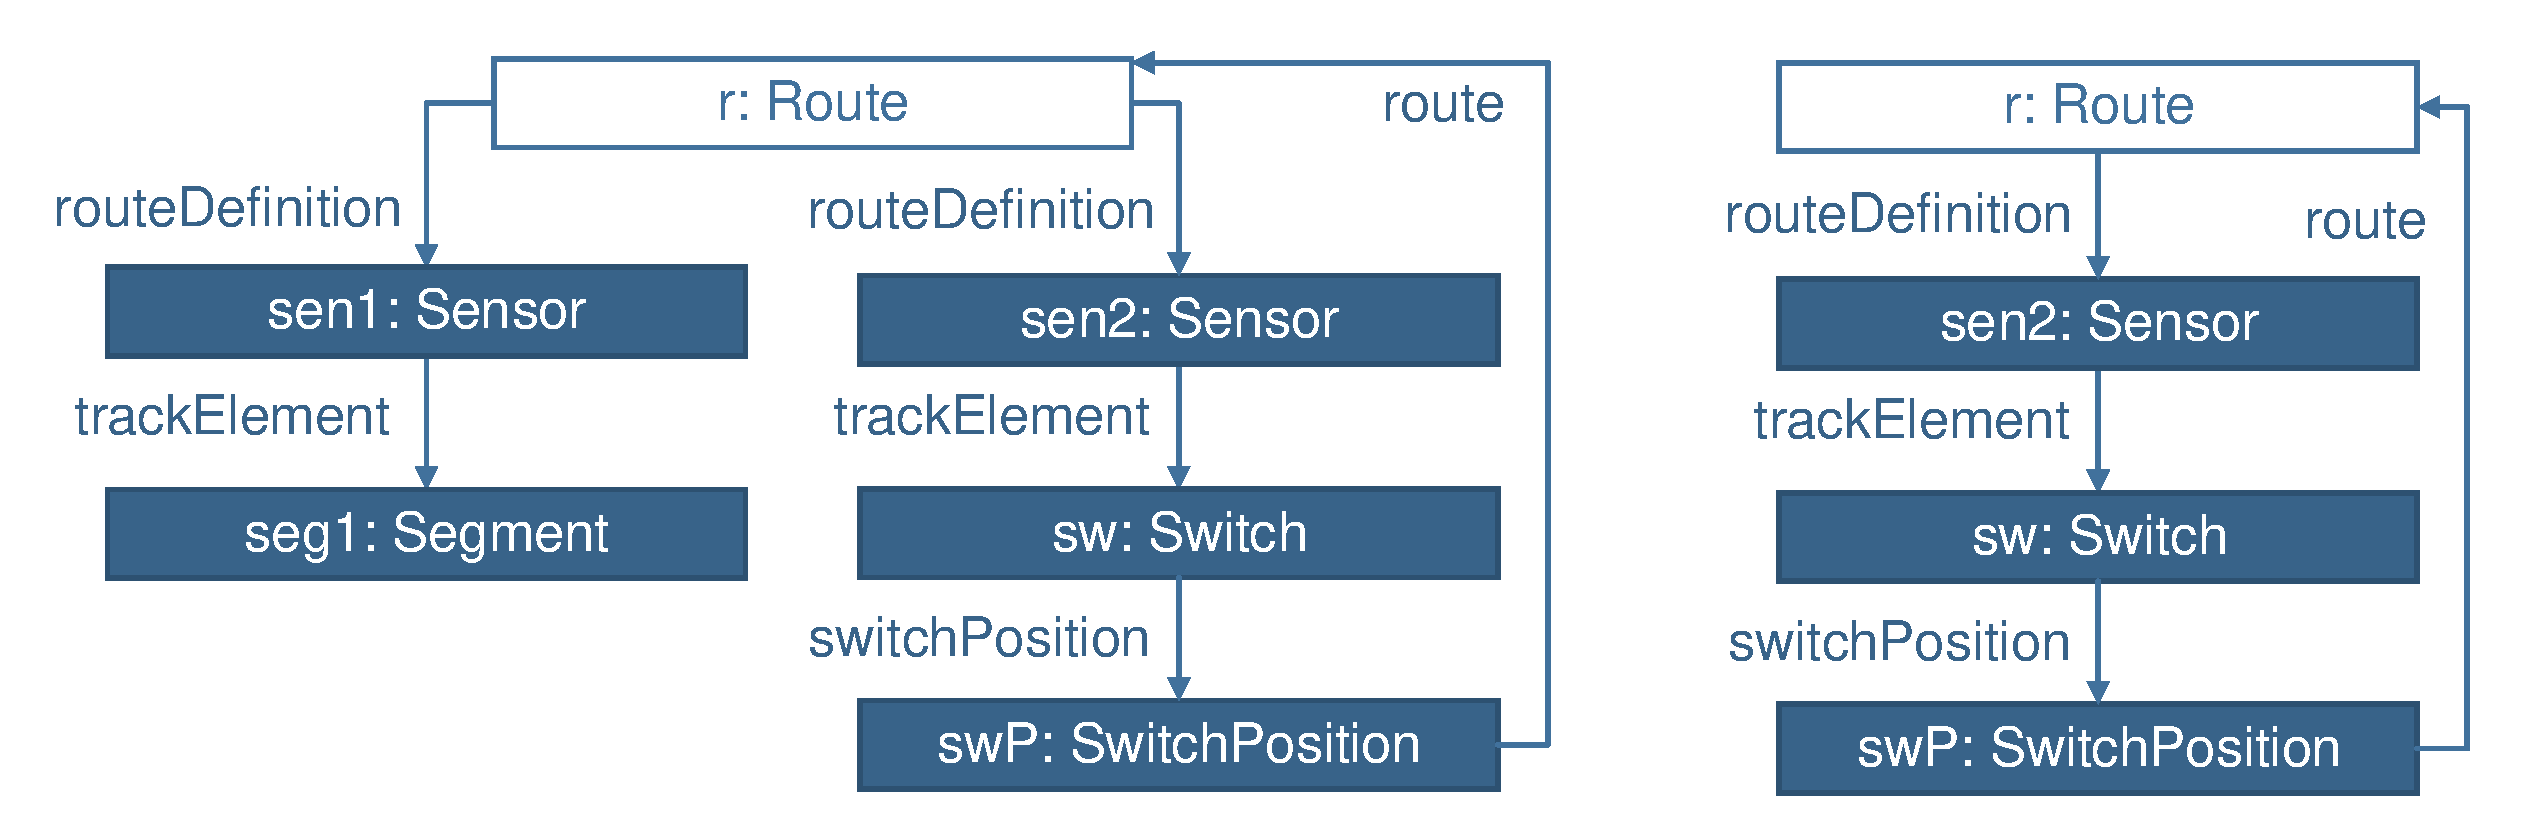
\includegraphics[scale=0.4]{figures/parameters.pdf}
    \caption{The \codeCap{Params} and \codeCap{ParamsCircle} pattern schemas (first step).}
    \label{fig:aseparams}
\end{center}
\end{figure}



\subsubsection{\code{Checks} Query Series for the \code{numAttrChecks} Metric}
Each \code{Checks} query use the same pattern body described by the pattern
schema in \figref{fig:asechecks}, but each one is extended with an increasing
number of attribute check constraints. These check constraints filter results
based on the \emph{year, height} and \emph{length} value of the segments \emph{seg1} and
\emph{seg2}, resulting in seven queries.

\begin{figure}[htb]
\begin{center}
    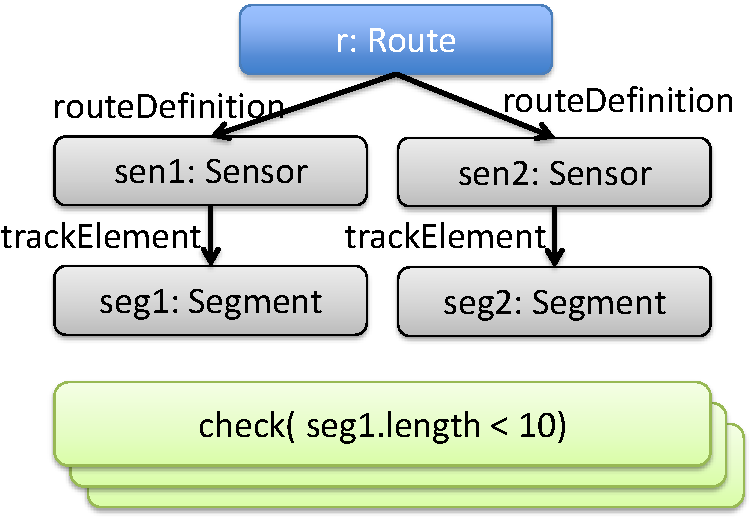
\includegraphics[scale=0.4]{figures/checks.pdf}
    \caption{The \codeCap{Checks} pattern schema.}
    \label{fig:asechecks}
\end{center}
\end{figure}


\subsubsection{\code{Negs} Query Series for the \code{nestedNacDepth} Metric}
\code{Negs} queries present increasing number of nested \emph{neg} constraints.
These queries are defined based on the following schema: at the bottom there is
a pattern checking for segments with length less than ten. Next, for each query
a new segment is matched, and the previous pattern is encapsulated in a negative
pattern call. $i=5$ queries are defined in the benchmark, described by the
schema in \figref{fig:asenegs}.

\begin{figure}[htb]
\begin{center}
    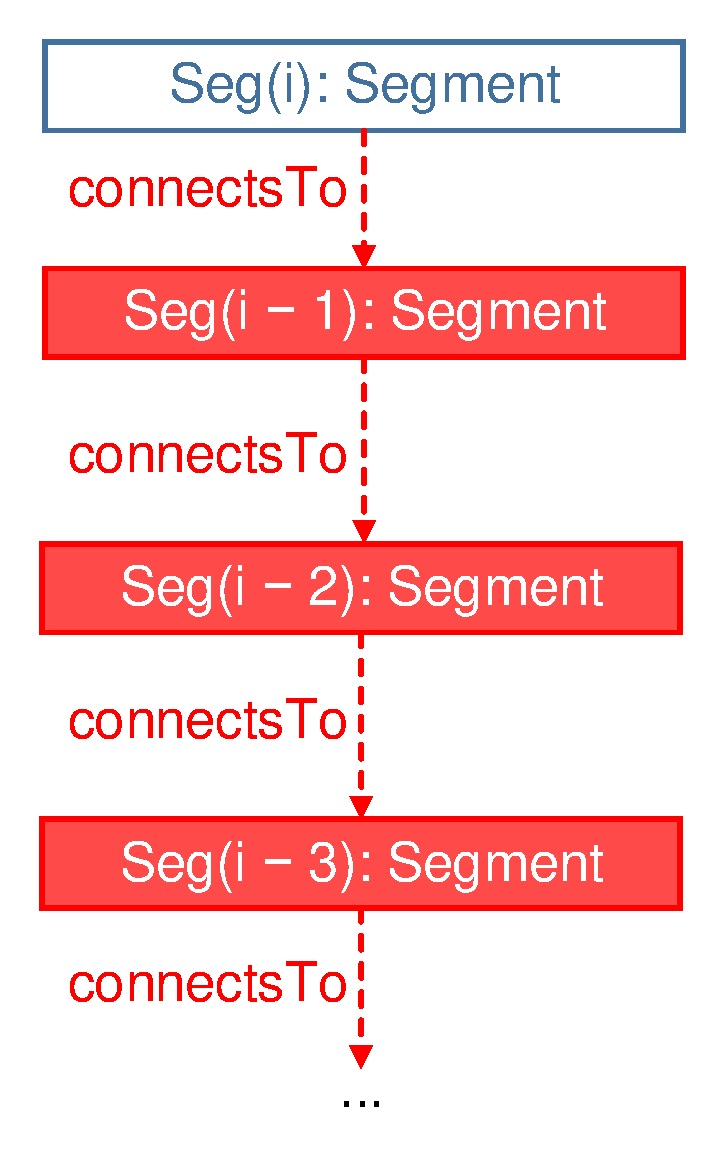
\includegraphics[scale=0.4]{figures/negs.pdf}
    \caption{The \codeCap{Negs} pattern schema.}
    \label{fig:asenegs}
\end{center}
\end{figure}

\begin{table}[htb]
	\centering
	\footnotesize
	\begin{tabular}{|l|c|c|c|c|c|}
	\hline 
	\textbf{Query series} & \textbf{numParameters} & \textbf{numVariables} &
	\textbf{numEdgeConstraints} & \textbf{numAttrChecks} &
	\textbf{nestedNacDepth}\\ \hline Param & \cellcolor{blue!25}1--5 & 8 & 8 & 0 & 0\\ \hline ParamCircle & \cellcolor{blue!25}1--5 & 6 & 6 & 0 & 0\\ \hline
	Locals & 1 & \cellcolor{blue!25}3--7 & 6 & 0 & 0\\ \hline
	Refs & 1 & 5 & \cellcolor{blue!25}4--7 & 0 & 0\\ \hline
	Checks & 1 & 5--11 & 4--10 & \cellcolor{blue!25}0--6 & 0\\ \hline
	Neg & 2--6 & 3--11 & 1--5 & 1 & \cellcolor{blue!25}0--10\\ \hline
	\end{tabular}
	\caption{Query-only metrics.}
	\label{tab:queryonlymetrics}
\end{table}


After the construction of the query series, we evaluated the query only metrics
on them. \autoref{tab:queryonlymetrics} shows the results of the evaluation:
each cell contains the value or range of values that we got on each query
series. This table confirms that there are query series for every metric (shown
in blue), and each query series differ in one or more metrics.

\subsection{Complex Analysis}
